\problemname{Inomhusorientering}
En snabbt växande sport är \emph{inomhusorientering}, där de största tävlingarna lockar tusentals deltagare som springer runt på t.ex. ett campus.
Genom arrangörens noga uttänkta avspärrningar blir det en labyrintliknande utmaning att ta sig mellan kontrollerna.
Ofta gäller det att optimera användandet av trappor, och det är det vi ska titta på i den här uppgiften.
Givet en karta som indelats i $N$ \emph{områden} ska du beräkna det minimala antalet trapplöpningar som orienteraren behöver göra för att besöka de $N$ områdena i tur och ordning (för att ta en kontroll i varje).


Byggnaden innehåller ett antal lodräta trapphus betecknade med bokstäver.
Varje område ligger på en viss våning och är kopplat till ett eller flera av trapphusen.
Ett trapphus behöver inte vara kopplat till något område på varje våning.
Exempelvis kan trappa B förbinda ett område på våning $1$ med ett annat område på våning $3$, utan att vara kopplad till något område på den mellanliggande våning $2$.
Att förflytta sig en våning upp eller ner i en trappa kostar en tidsenhet.
Däremot bryr vi oss inte om tiden det tar att röra sig inom ett område och hitta kontrollen.

\section*{Indata}
Den första raden innehåller heltalet $N$ ($3\le N \le 15$), antalet områden.

Detta följs av en rad för varje område.
En rad innehåller först våningen som området befinner sig på (ett heltal mellan $1$ och $100$) följt av en sträng som innehåller ett eller flera tecken, valda bland \texttt{A-Z}, och som anger vilket eller vilka trapphus området är kopplat till.

\section*{Utdata}
Skriva ut ett enda tal: den minimala tiden det tar att besöka de $N$ områdena i precis den ordning de angavs i indata, med starten i område $1$ och målet i område $N$. 

\section*{Poängsättning}
Din lösning kommer att testas på en mängd testfallsgrupper.
För att få poäng för en grupp så måste du klara alla testfall i gruppen.

\noindent
\begin{tabular}{| l | l | p{12cm} |}
  \hline
  \textbf{Grupp} & \textbf{Poäng} & \textbf{Gränser} \\ \hline
  $1$    & $20$      & Alla strängar kommer vara A \\ \hline
  $2$    & $80$      & Inga ytterligare begränsningar. \\ \hline
\end{tabular}

\section*{Förklaring av exempelfall}
\begin{figure}[h]
  \centering
  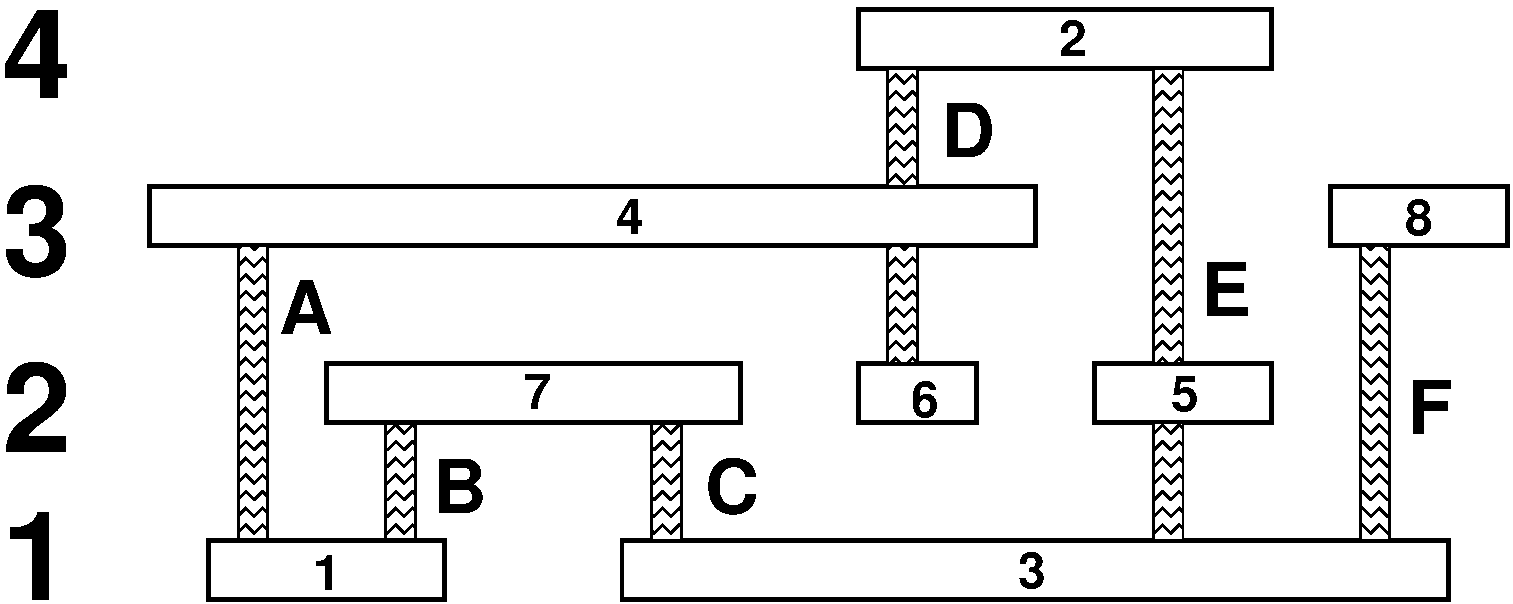
\includegraphics[width=0.6\textwidth]{orient.pdf}
  \caption{
    Genomskärning av byggnaden i exempel 2.
    De stora siffrorna visar våningsnummer, de små numreringen av områdena. En möjlig kortaste väg genom hela banan är:\\
  }
\end{figure}
I det andra exemplet finns en väg med 24 steg: AAD -- EEE -- CBAA -- DEE -- EEDD -- DAAB -- CFF (bokstäverna indikerar vilken trappa som användes i varje steg).
